\chapter{Narzędzia i algorytmy}
\label{chapter:2}

W niniejszym rozdziale opisane są wybrane algorytmy służące do klasyfikacji binarnej --- las losowy, maszyna wektorów nośnych, sieci konwolucyjne oraz rekurencyjna sieć LSTM (długoterminowa pamięć krótkoterminowa). Dla każdego algorytmu opisana jest jego konstrukcja i właściwości, a także szczegóły implementacji na potrzeby niniejszej pracy.

\section{Las losowy}
\label{sec:rf}

Las losowy to szeroko wykorzystywana metoda uczenia maszynowego, mogąca posłużyć do rozwiązania problemu klasyfikacji. Polega ona na wytrenowaniu wielu drzew decyzyjnych na losowych podzbiorach danych wejściowych. W celu uzyskania predykcji, sprawdzane są predykcje tak uzyskanych drzew --- predykcja lasu to klasa wybrana przez większość drzew w lesie. Las losowy ma lepsze możliwości dostosowania się do danych wejściowych niż prostsze modele (np. liniowe), ale jest bardziej odporny na przetrenowanie (\textit{overfitting}) niż drzewo decyzyjne.
W tej sekcji opisana jest metoda drzewa decyzyjnego, następnie konstrukcja lasu losowego, potem omówione są kluczowe właściwości lasu losowego, zaś na końcu szczegóły implementacji algorytmu na potrzeby niniejszej pracy.

\subsection{Drzewo decyzyjne}
\label{subsec:dt}

Drzewo decyzyjne to jedna z podstawowych metod wykorzystywana w data miningu dla klasyfikacji \cite{rokach2007data}. Polega ona na zbudowaniu modelu predykcyjnego, który ma postać ukorzenionego drzewa. Każdy wewnętrzny węzeł drzewa jest oznaczony którymś z atrybutów z danych wejściowych. Każda z krawędzi wychodzących z węzła do potomka jest oznaczona zakresem wartości tego atrybutu. Każdy liść drzewa jest oznaczony jedną z klas, które model ma przewidywać. Predykcja za pomocą tego modelu polega na przejściu po drzewie od korzenia aż do któregoś z liści, po drodze wybierając odpowiednie krawędzie w zależności od wartości odpowiednich atrybutów próbki wejściowej.

\begin{figure}[H]
	\centering
	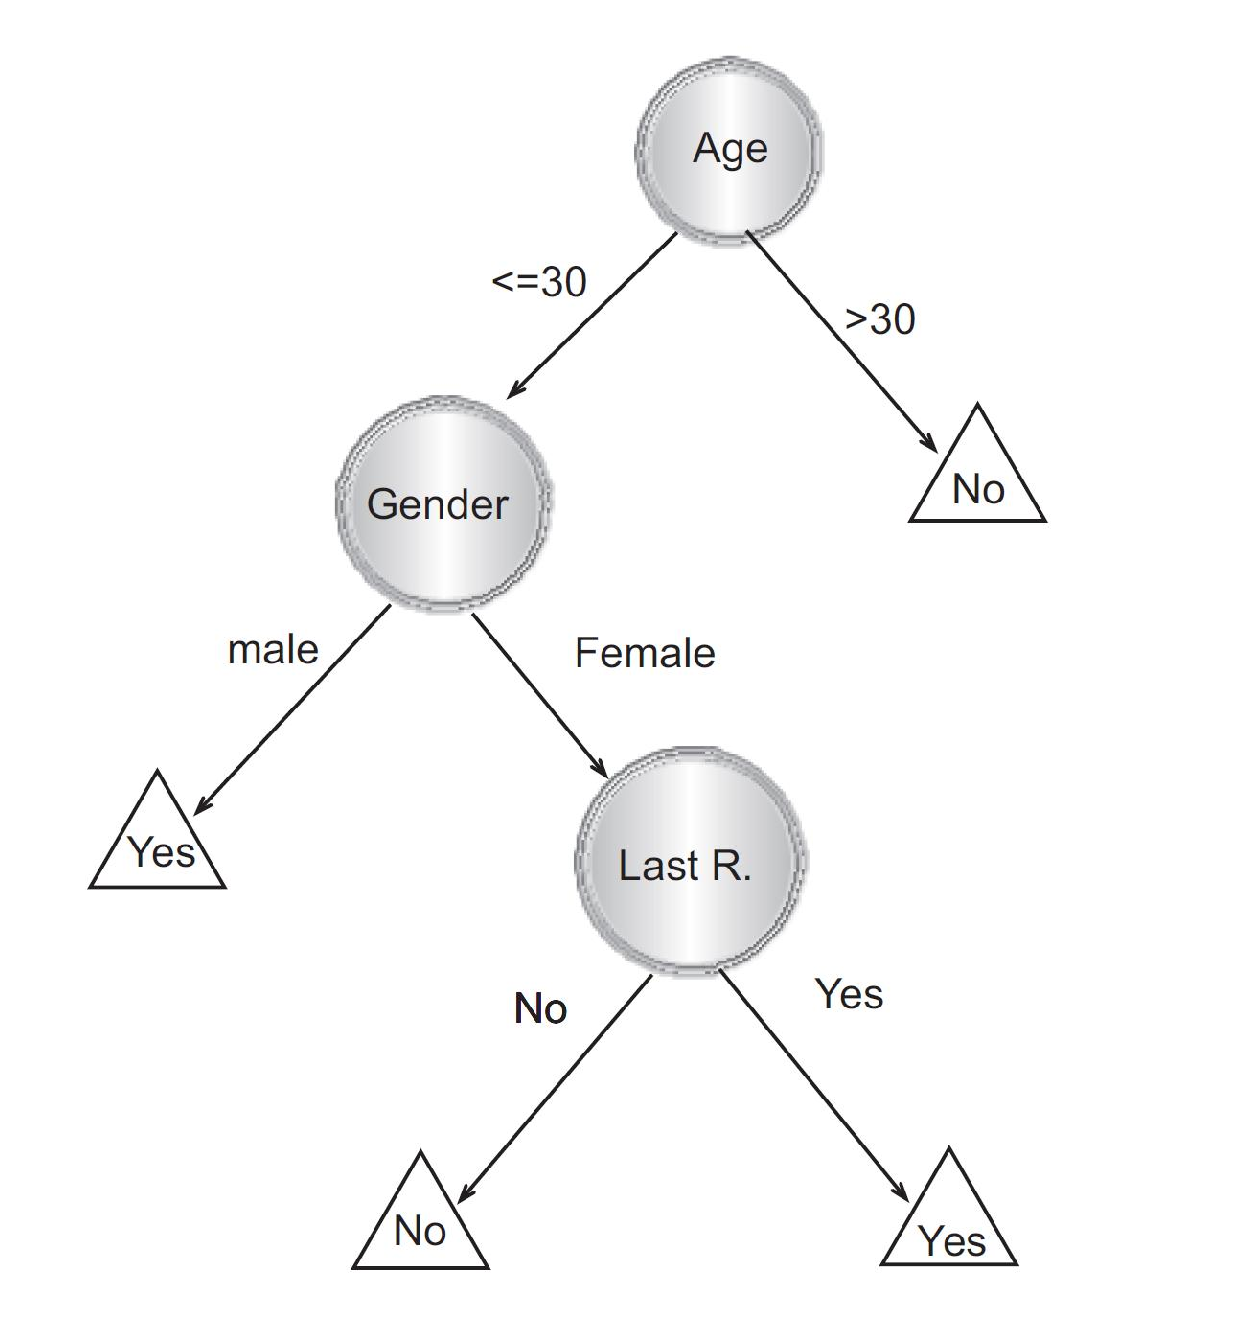
\includegraphics[width=0.6\linewidth]{images/chapter2/decision_tree.pdf}
	\caption{Drzewo decyzyjne \cite{rokach2007data}}
	\label{fig:decision-tree}
\end{figure}
Budowa drzewa decyzyjnego odbywa się typowo za pomocą algorytmu zachłannego. W danym wierzchołku wybierany jest ten atrybut oraz takie zakresy, które w wyniku podzielenia zbioru wejściowego stworzą podzbiory możliwie najbardziej jednorodne ze względu na klasy w nich zawarte. Ściślej, jako metrykę jakości danego podziału stosuje się zwykle miarę \textit{Information Gain} bądź \textit{Gini Impurity} --- wybór konkretnej miary jest hiperparametrem algorytmu uczącego, jednakże publikacje wskazują na to, że obie miary dają podobne wyniki \cite{tangirala2020evaluating}. Utworzone podzbiory przekazywane są rekurencyjnie w głąb drzewa w celu utworzenia kolejnych potomków. Procedura trwa do momentu gdy w każdym wierzchołku są już próbki z tylko jednej klasy, lub gdy zostanie osiągnięta maksymalna głębokość drzewa --- hiperparametr algorytmu.
Jak widać z konstrukcji modelu, drzewo decyzyjne ma bardzo wysoką interpretowalność --- łatwo zrozumieć w jaki sposób obliczona została dana predykcja. Drzewo decyzyjne charakteryzuje się też tym, że ma możliwość idealnego dopasowania się do danych treningowych. Często skutkuje to przeuczeniem się (\textit{overfitting}) i słabymi wynikami na danych testowych.

\subsection{Konstrukcja lasu losowego}

Las losowy budowany jest poprzez stworzenie pewnej liczby drzew decyzyjnych --- liczba drzew jest hiperparametrem algorytmu. Każde z drzew jest budowane na podstawie losowo stworzonego podzbioru zbioru treningowego. Ściślej, używana jest technika o nazwie \textit{bagging} (od ang. \textit{Bootstrap aggregating}) \cite{breiman1996bagging} --- dla zbioru wejściowego o rozmiarze $n$, dla każdego drzewa losowane jest ze zwracaniem $n$ próbek ze zbioru.
\\Dodatkowo, podczas budowy pojedynczych drzew, przy wybieraniu atrybutu do podziału w węźle drzewa, każdorazowo przeglądany jest jedynie losowy podzbiór atrybutów. Typowo losuje się $\sqrt{p}$ gdzie p to liczba atrybutów.
\\Tak zbudowany las wykorzystuje się do predykcji w następujący sposób --- dla danej próbki oblicza się predykcję z każdego z drzew, a następnie sprawdza się która z klas została przewidziana najczęściej.

\subsection{Właściwości}

Las losowy ma podobną siłę wyrazu jak drzewo decyzyjne. Jest jednak dużo bardziej odporny na przeuczenie --- innymi słowy ma mniejszą wariancję ale podobne obciążenie (\textit{bias}). Dzieje się tak dzięki temu, że drzewa są trenowane niezależnie --- czyni to model dużo mniej czułym na szum w zbiorze treningowym. Używanie podzbioru atrybutów podczas budowy węzłów ma za zadanie dodatkowego zmniejszenia korelacji między drzewami (w przeciwnym przypadku wszystkie stworzone drzewa będą preferowały atrybuty będące najsilniejszymi predyktorami, co sprawi, że będą one podobne) \cite{ho2002data}.
\\Las losowy jest też używany dla oszacowania ważności poszczególnych atrybutów --- podczas konstrukcji drzew, można zaobserwować jaka była miara jednorodności atrybutów użytych w węzłach. Tak stworzony ranking ważności atrybutów może pomóc w zinterpretowaniu zbioru danych, lub w wyborze najważniejszych atrybutów do innego algorytmu.

\subsection{Implementacja}

W ramach niniejszej pracy użyłyśmy implementacji lasu losowego dla języka Python zawartej w klasie \verb_sklearn.ensemble.RandomForestClassifier_ z biblioteki \verb_scikit-learn_. Pozwala ona na zdefiniowanie kluczowych hiperparametrów oraz na ekstrakcję ważności atrybutów.


\subsubsection {Wybór hiperparametrów}
\label{subsub: hyperparameters}

Do znalezienia hiperparametrów modelu (liczba drzew, maksymalna głębokość pojedynczego drzewa) użyłyśmy klasy \verb_RandomizedSearchCV_ z biblioteki
\verb_sklearn_ z pakietu \verb_model_$\_$\verb_selection_, która pozwala na przeszukiwaniu przestrzeni hiperparametrów na zdefiniowanym przez nas zakresie w efektywny sposób przy użyciu techniki walidacji krzyżowej (\textit{cross-validation}). Technika ta polega na wydzieleniu części danych treningowych, wytrenowaniu na nich modelu a następnie sprawdzeniu wyników predykcji na pozostałej części danych treningowych (zbiorze walidacyjnym). 

Użyta przez nas metoda używa techniki \textit{5-fold cross validation}, która polega na podzieleniu danych treningowych na 5 części, a następnie pięciokrotnym powtórzeniu procedury walidacji krzyżowej (tak, aby każda z 5 części raz została użyta jako zbiór walidacyjny). Wyniki wszystkich eksperymentów są zapisywane w klasie wraz z ich najistotniejszymi miarami statystycznymi (średnia wyników, odchylenie standardowe, średni czas trenowania modelu) oraz rankingowane.
\\\verb_RandomizedSearchCV_ jest przydatnym narzędziem, gdy chcemy przeszukać duży zbiór hiperparametrów i czas trenowania modelu jest długi. Nie sprawdza ona wszelkich możliwych kombinacji, tylko trenuje model na losowo wybranych hiperparametrach z podanych przez nas przedziałów, rozkładów lub zbiorów. 


\section{Maszyna wektorów nośnych}
\label{sec:svm}

Maszyna wektorów nośnych (\textit{Support Vector Machine}, SVM) \cite{cortes1995support}, jest to jeden z klasycznych algorytmów klasyfikacji binarnej. Opiera się on na znalezieniu hiperpłaszczyzny rozdzielającej przestrzeń danych wejściowych na dwie klasy, w taki sposób by odległość punktów danych od hiperpłaszczyzny była jak największa.

W tej sekcji opisana jest konstrukcja maszyny wektorów nośnych, następnie opisane są właściwości modelu, a na końcu szczegóły implementacji algorytmu na potrzeby niniejszej pracy.

\subsection{Konstrukcja}

Dane wejściowe o $p$ atrybutach można traktować jako zbiór punktów w $p$-wymiarowej przestrzeni --- każdy o przypisanej klasie. Maszyna wektorów nośnych to metoda znalezienia takiej $(p-1)$-wymiarowej płaszczyzny, która będzie rozdzielać punkty z jednej klasy od punktów z drugiej klasy. W przypadku gdy istnieje wiele takich płaszczyzn, wybierana jest taka, która maksymalizuje odległość najbliższych jej punktów. W przypadku gdy nie istnieje taka płaszczyzna, wybierana jest taka, która minimalizuje dodatkowo odległość od niej błędnie sklasyfikowanych punktów. To w jakim stosunku optymalizować te dwa cele jest hiperparametrem algorytmu (dalej oznaczony $\lambda$). 

\begin{figure}[H]
	\centering
	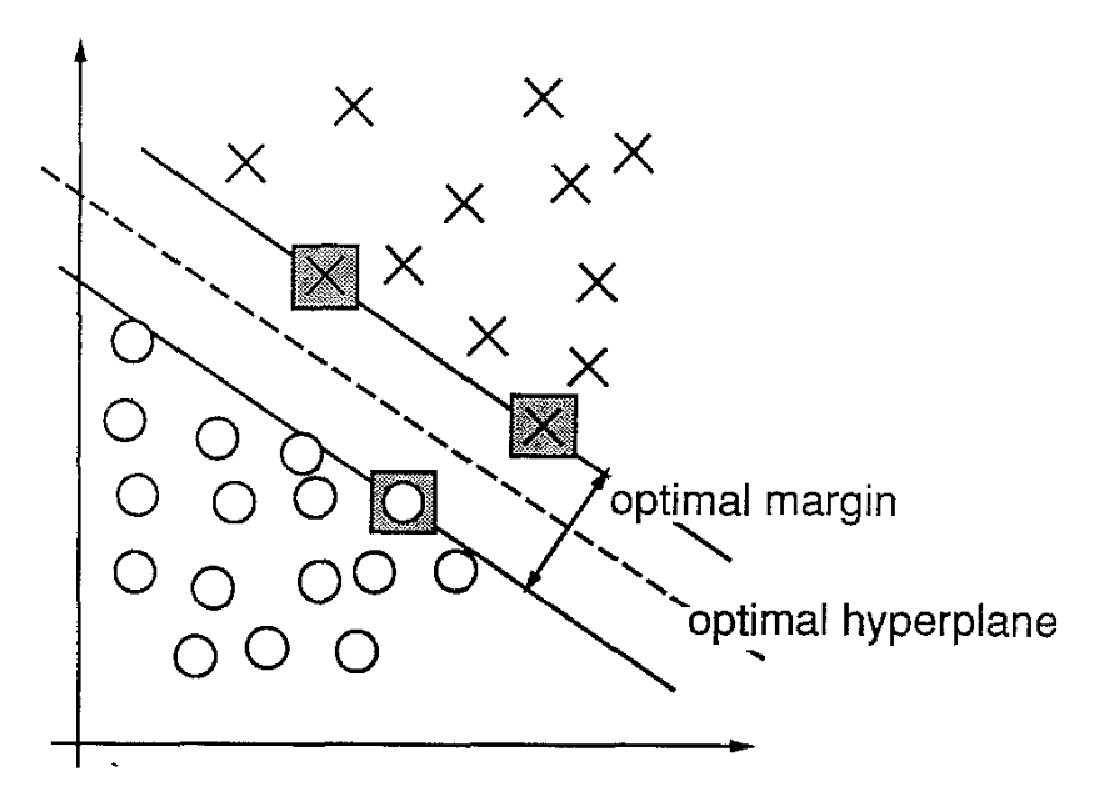
\includegraphics[width=0.6\linewidth]{images/chapter2/SVM.pdf}
	\caption{Przykład rozdzielonych punktów w 2-wymiarowej przestrzeni --- wektory nośne oznaczone są kwadratami \cite{cortes1995support}}
	\label{fig:svm}
\end{figure}
\noindent Wyraźmy hiperpłaszczyznę za pomocą jej wektora normalnego w oraz liczby $b$:
\begin{equation}
w^Tx - b = 0 
\end{equation}

\noindent Znalezienie odpowiedniej hiperpłaszczyzny sprowadza się do minimalizacji funkcji kosztu $f(w,b)$
\begin{equation}
\left[ \frac{1}{n}\sum_{i=1}^n \max(0, 1 - y_{i}(w^Tx_{i} - b))\right] + \lambda ||w|| ^2
\end{equation}

\noindent gdzie $n$ to liczba punktów, $x_i$ to $i$-ty punkt danych, $y_i$ to wartość jego klasy ($1$ lub $-1$), a $\lambda$ to hiperparametr algorytmu.
\\Pierwszy człon wyraża karę za źle sklasyfikowane punkty (tym większą im dalej są od hiperpłaszczyzny). Drugi człon jest odwrotnie proporcjonalny do kwadratu odległości hiperpłaszczyzny od poprawnie sklasyfikowanych punktów.

\subsection{Właściwości}

Maszyna wektorów nośnych w opisanej postaci tworzy model liniowy, charakteryzuje się więc wysokim obciążeniem (\textit{bias}) i niską wariancją. W sytuacjach gdzie klasy nie są łatwo separowalne liniowo, często stosuje się tzw. kernel trick przekształcający nieliniowo oryginalną przestrzeń punktów \cite{aizerman1964theoretical}.

\subsection{Implementacja}

W ramach niniejszej pracy użyłyśmy klasycznej implementacji maszyny wektorów nośnych dla języka Python zawartej w klasie \verb_sklearn.svm.LinearSVC_ z biblioteki \verb_scikit-learn_. Pozwala ona na zdefiniowanie hiperparametru $C = 1/ \lambda$.
\\Do znalezienia parametru \textit{C} użyłyśmy klas z biblioteki \verb_sklearn.model_$\_$\verb_selection_ - \verb_RandomizedSearchCV_ opisanej powyżej (Sekcja. \ref{subsub: hyperparameters}) oraz \verb_GridSearchCV_  
która również używa techniki walidacji krzyżowej, jednak sprawdza wszystkie możliwe kombinacje ze zdefiniowanych przez nas zbiorów. 


\section{Konwolucyjna sieć neuronowa}
\label{sec:cnn}
Konwolucyjna sieć neuronowa (\textit{Convolutional Neural Network}) to rodzaj sztucznej sieci neuronowej. Jej konstrukcja jest inspirowana procesami biologicznymi zachodzącymi w korze wzrokowej w mózgu \cite{chauhan2018convolutional}. Typowo sieci konwolucyjne wykorzystuje się do zadań uczenia maszynowego związanego z rozpoznawaniem obrazów. Mogą być jednak stosowane także w innych dziedzinach, w szczególności w przetwarzaniu języka naturalnego.

W tej sekcji najpierw opisany jest koncept klasycznej sieci neuronowej. Następnie opisana jest konstrukcja konwolucyjnej sieci, oraz zastosowanie jej w przetwarzaniu języka naturalnego. Na końcu podane są szczegóły implementacji sieci na potrzeby niniejszej pracy.

\subsection{Sieci neuronowe}
\label{subsec:nn}

Klasyczna wielowarstwowa sieć neuronowa składa się z sekwencji warstw, w których znajduje się duża liczba węzłów obliczeniowych (tzw. neuronów). Pojedynczy neuron przyjmuje na wejściu wektor liczb rzeczywistych $x$, do którego następnie aplikowany jest wektor wag $w$ (wynik uczenia sieci) przypisany do tego neuronu.
W wyniku otrzymywana jest liczba:

\begin{equation}
a = \sum_{i=1}^n w_i x_i
\end{equation}

\noindent do której aplikowana jest funkcja aktywacji --- decydująca o tym, jaki wynik zostanie przekazany do kolejnej warstwy \cite{gurney2013introduction}. Funkcje aktywacji odgrywają ważną rolę w sieciach neuronowych --- pozwalają dodać nieliniowość --- bez ich użycia, wynik wyjściowy modelu byłby kombinacją liniową danych wejściowych, z ograniczonymi możliwościami modelowania skomplikowanych typów danych (takich jak obrazy czy język naturalny) \cite{sharma2017activation}.  

\begin{figure}[H]
	\centering
	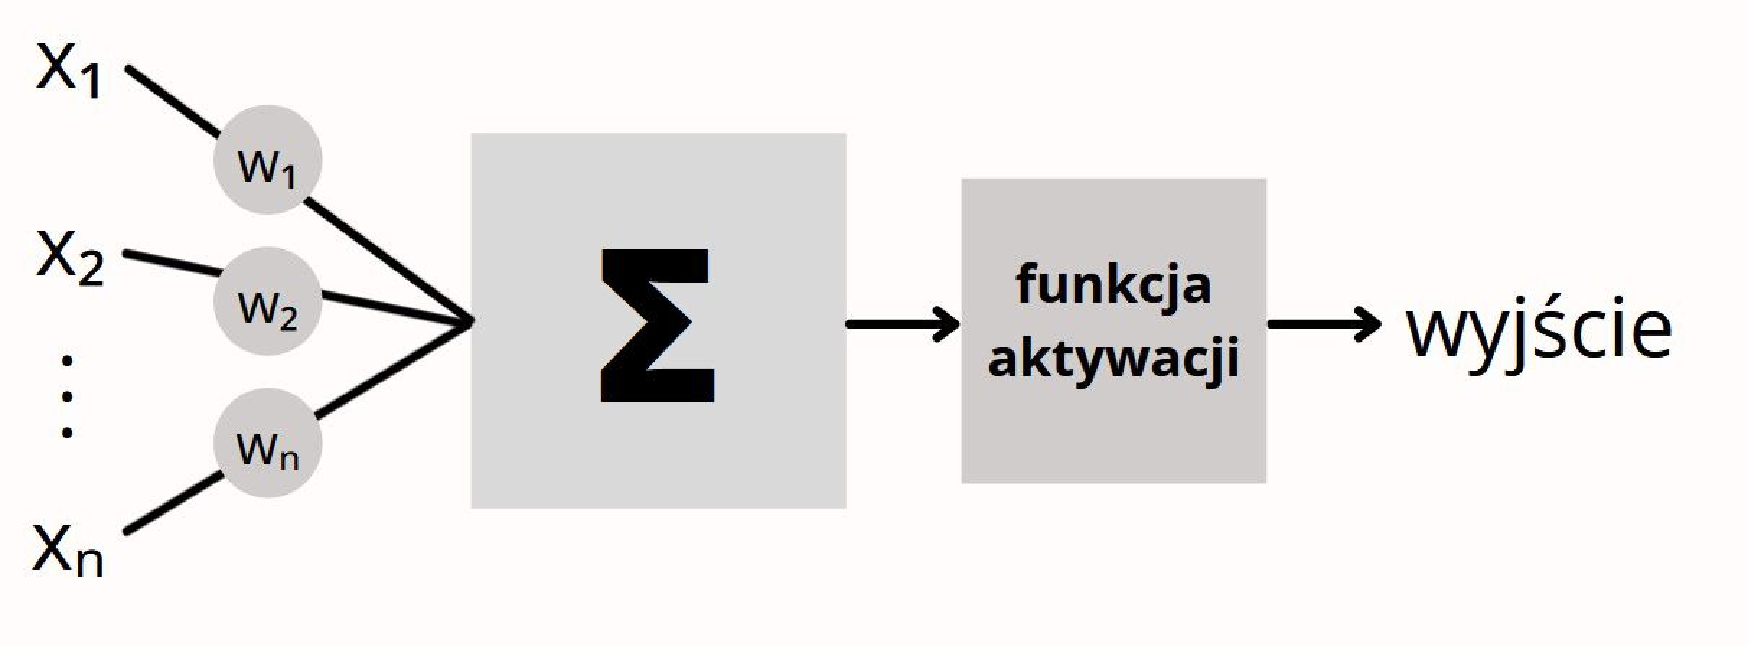
\includegraphics[width=0.6\linewidth]{images/chapter2/perceptron.pdf}
	\caption{Schemat działania pojedynczego neuronu}
	\label{fig:perceptron}
\end{figure}

\noindent Pierwsza warstwa nazywana jest warstwą wejściową (\textit{input layer}), która przyjmuje na wejściu czyste dane w postaci wektorów. Kolejne warstwy to warstwy ukryte (\textit{hidden layers}), do których wejściami są wyniki przekazane przez neurony poprzedniej warstwy. Ostatnią warstwą jest warstwa wyjściowa (\textit{output layer}), która na wejściu również przyjmuje dane z poprzedniej warstwy, a której wyjcie jest predykcją modelu.

\begin{figure}[H]
	\centering
	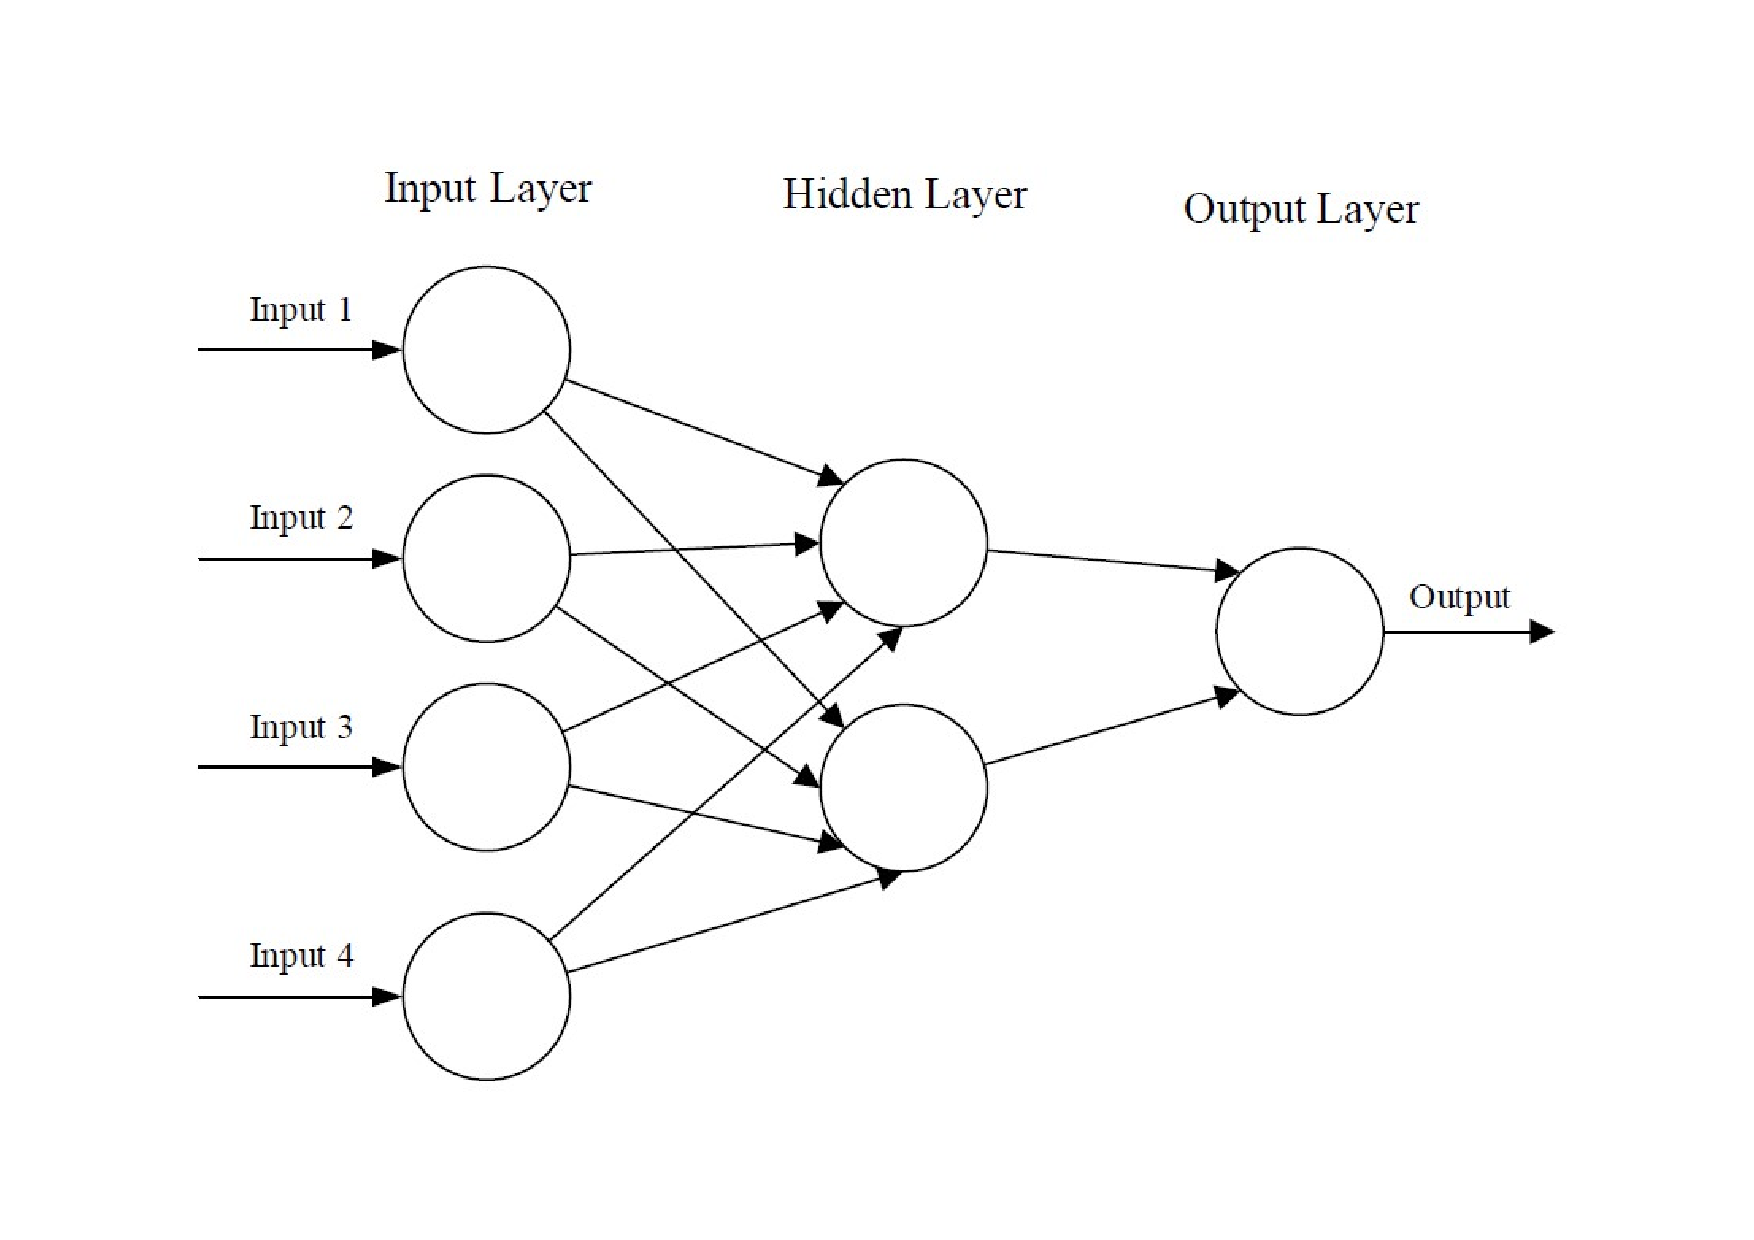
\includegraphics[width=0.9\linewidth]{images/chapter2/ann-layers.pdf}
	\caption{Wielowarstwowa sieć neuronowa \cite{o2015introduction}}
	\label{fig:ann-layer}
\end{figure}

\noindent Istnieje wiele różnych funkcji aktywacji, z których najpopularniejsze opisane są w \cite{sharma2017activation}. W ramach niniejsze pracy wykorzystałyśmy następujące funkcje:
\begin{enumerate}
	\item Funkcja sigmoidalna
	\begin{equation}
	f(x) = \frac{1}{1 + e^{-x}}
	\end{equation}
	
	Funkcja ta, mapująca liczby rzeczywiste na przedział $(0, 1)$, jest jedną z najczęściej stosowanych w sieciach neuronowych.
	
	\item Funkcja ReLU (od ang. \textit{rectified  linear  unit}) 
	\begin{equation}
	f(x) = \max(0,x)
	\end{equation}
	
	Funkcja ta jest szeroko stosowana w warstawch ukrytych m.in. dzięki prostocie obliczeń oraz rozrzadzeniu aktywnych neuronów (neurony aktywują się tylko dla $a > 0$).
	
\end{enumerate}

\subsection{Trening sieci neuronowej}

Trening --- uczenie sieci neuronowej ma na celu zminimalizowanie obserwowanego błędu, czyli różnicy między predykcją sieci na danych treningowych a faktycznymi klasami. Sieć inicjalizuje się z losowymi wagami. Następnie sieć jest aplikowana do danych wejściowych i wagi są aktualizowane w celu zmniejszeniu uzyskanego błędu. Proces powtarzany jest iteracyjnie. \cite{gurney2013introduction}. Hiperparametrami modelu są liczba iteracji (epok) oraz ile próbek naraz używać podczas jednego kroku aktualizacji (wielkość wsadu, \textit{batch size}).
\\Aktualizacja wag odbywa się za pomocą procesu zwanego propagacją wsteczną (\textit{backpropagation})  \cite{goodfellow2016deep}. Wagi aktualizowane są w kierunku gradientu funkcji błędu w zależności od tych wag. Innymi słowy, wartość błędu jest dzielona proporcjonalnie pomiędzy wagi które za niego odpowiadają.
\\W celu przeciwdziałania przeuczeniu się sieci neuronowej, można wykorzystać technikę zwaną \textit{dropout} \cite{srivastava2014dropout}. Polega ona na zignorowaniu podczas obliczania predykcji na potrzeby treningu niektórych neuronów z prawdopodobieństwem $p$ będącym hiperparametrem. Dzięki temu że żaden neuron nie jest trenowany na całym zbiorze treningowym, sieć będzie miała mniejszą skłonność do przeuczenia się.

\subsection{Sieci konwolucyjne}
\label{subsec:cnn}

Sieci konwolucyjne są modyfikacją sieci neuronowych, stworzone z myślą o przetwarzaniu obrazów. Wejściem do sieci konwolucyjnej jest trójwymiarowa macierz: typowo jest to dwuwymiarowy obrazek, gdzie każdy piksel opisany jest trzema wartościami --- R, G, B. Podobnie jak w przypadku sieci neuronowych, sieć konwolucyjna składa się z sekwencji warstw.

Pojedyncza warstwa konwolucyjna składa się z pewnej liczby (hiperparametr) filtrów. Każdy filtr to trójwymiarowa macierz wag. Wysokość i szerokość filtra (hiperparametry) powinny być mniejsze niż odpowiednio wysokość i szerokość wejścia, natomiast głębokość musi być równa głębokości wejścia. Zaaplikowanie filtru do macierzy wejściowej polega na “przyłożeniu” go do każdej możliwej pozycji $x$,$y$ wejścia, i obliczeniu iloczynu skalarnego filtra i odpowiedniego wycinka wejścia. W wyniku tej aplikacji powstaje dwuwymiarowa macierz zawierająca iloczyny skalarne, o wysokości i szerokości równych wysokości i szerokości wejścia (aby nie tracić informacji o pikselach znajdujących się na rogach obrazkach, często stosuje się technikę nazywaną \textit{zero-padding} --- jej szczegółowy opis można znaleźć w \cite{albawi2017understanding}. Wyniki aplikacji wszystkich filtrów z warstwy razem tworzą macierz trójwymiarową, która służy jako wejście do kolejnej warstwy.

\begin{figure}[H]
	\centering
	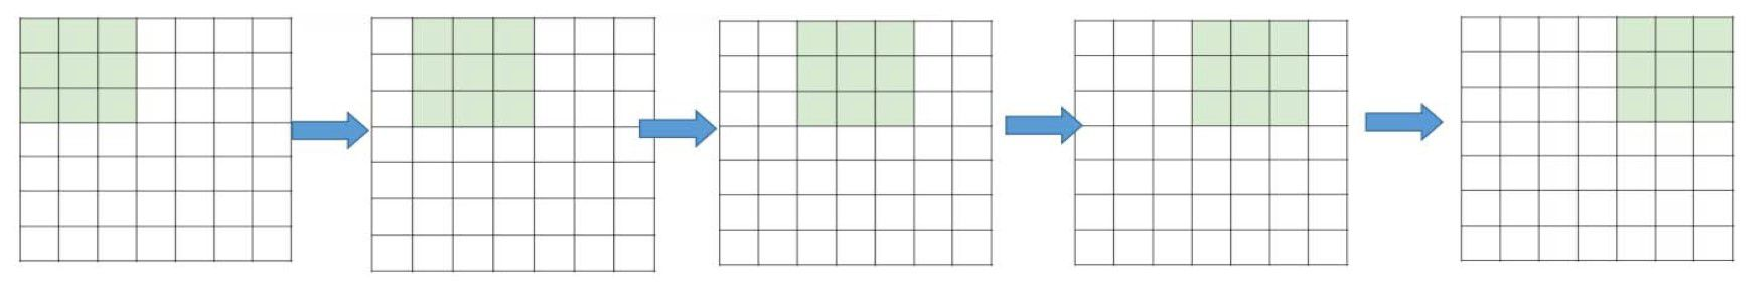
\includegraphics[width=0.8\linewidth]{images/chapter2/filter.pdf}
	\caption{Zastosowanie filtra w sieci konwolucyjnej \cite{albawi2017understanding}}
	\label{fig:filter}
\end{figure}

\noindent Oprócz warstw konwolucyjnych, stosuje się też inne rodzaje warstw. Jedną z nich jest warstwa typu \textit{pooling}. Jej zadaniem jest zmniejszenie wymiarowości danych płynących przez sieć. W tym celu segmenty wejścia są agregowane, na przykład poprzez branie maksimum z ich wartości \cite{albawi2017understanding}.

Architektura sieci konwolucyjnej typowo składa się z kilku warstw konwolucyjnych przeplatanych z warstwami \textit{pooling}, a następnie kilku warstw klasycznych sieci neuronowych, w tym kontekście nazywanych warstwami \textit{fully connected}. Trójwymiarowa macierz wychodząca z warstwy konwolucyjnej jest spłaszczana do jednowymiarowego wektora w celu przekazania jej do warstwy \textit{fully connected}.

\begin{figure}[H]
	\centering
	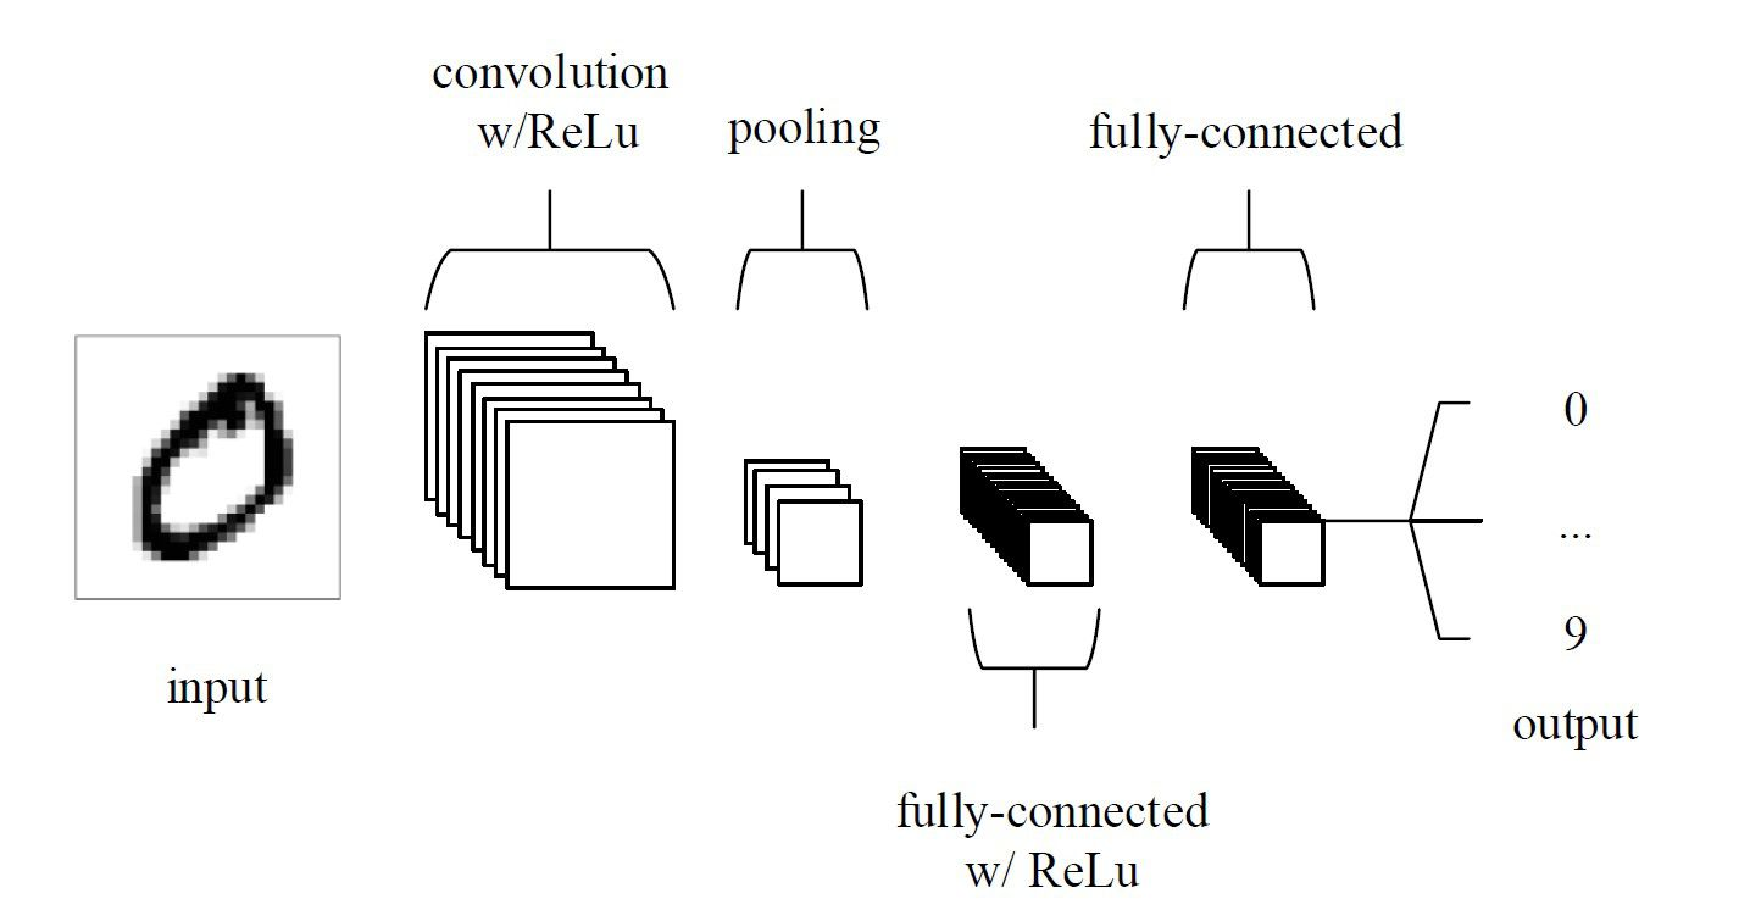
\includegraphics[width=0.8\linewidth]{images/chapter2/layered-conv.pdf}
	\caption{Pięciowarstwowa sieć konwolucyjna \cite{o2015introduction}}
	\label{fig:layered-conv}
\end{figure}

\subsection{Wykorzystanie sieci konwolucyjnych w przetwarzaniu języka naturalnego}
\label{subsec:word2vec}

Choć sieci konwolucyjne wymyślone zostały z intencją przetwarzania obrazów, w ostatnich latach wielokrotnie były wykorzystywane do przetwarzania tekstu \cite{minaee2019deep}. Wymaga to najpierw zanurzenia (\textit{embedding}) słów --- wyrażenia każdego słowa w postaci wektora liczb. Można wykorzystać do tego metodę Word2Vec \cite{mikolov2013efficient}. Polega ona na wytrenowaniu sieci neuronowej na korpusie tekstów, która dla danego słowa zwraca wektor liczb. Sieć trenowana jest w ten sposób, by wektory słów występujących w podobnym kontekście znajdowały się blisko siebie.

\begin{figure}[h]
	\centering
	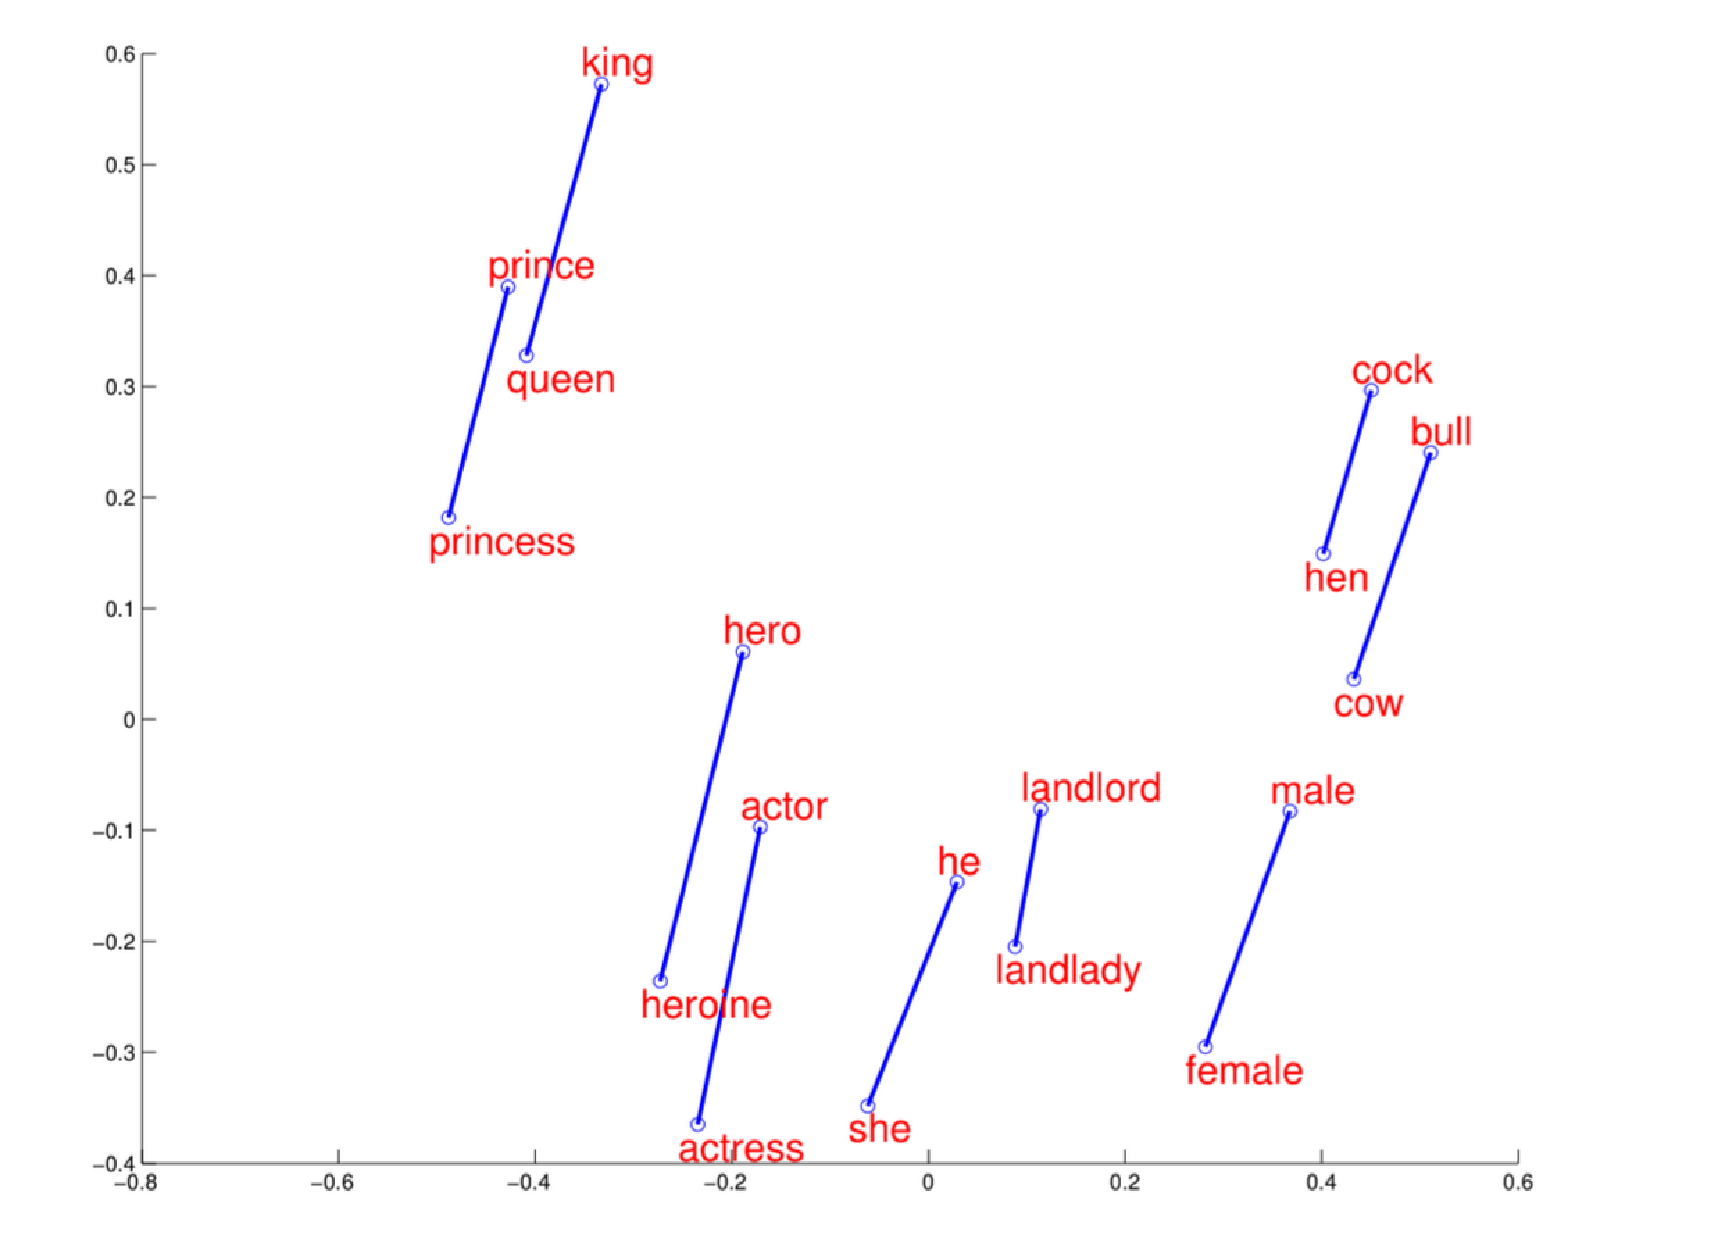
\includegraphics[width=0.8\linewidth]{images/chapter2/w2vpng.pdf}
	\caption{\href{https://drive.google.com/file/d/0B7XkCwpI5KDYRWRnd1RzWXQ2TWc/edit?resourcekey=0-oGRnY6qG7yWEqCXOHFKPcw}
		{Wizualizacja działania metody Word2vec}}
	\label{fig:word2vec}
\end{figure}

W przypadku tekstu, wejściem dla sieci konwolucyjnej będzie macierz nie trójwymiarowa, a dwuwymiarowa. Zamiast dwuwymiarowego obrazu używany jest jednowymiarowy tekst. Podczas gdy w przypadku obrazów każdy piksel reprezentowany jest za pomocą trzech liczb (R, G, B), każde słowo tekstu wejściowego jest wyrażone odpowiadającym mu wektorem zanurzenia.

W przypadku obrazów, pojedynczy filtr aplikowany jest do pikseli znajdujących się blisko siebie. Intuicyjnie, każdy piksel należy interpretować w kontekście jego otoczenia. W przypadku tekstów, analogicznie filtr aplikowany jest do słów znajdujących się blisko siebie. Jedyną różnicą jest że dla obrazów otoczenie ma dwa wymiary --- szerokość i wysokość, zaś dla tekstów jest to tylko jeden wymiar.

\subsection{Implementacja}

\subsubsection{Word2Vec}
\label{subsubsec:w2v}

W niniejszej pracy w stworzenia wektorów używanych do reprezentacji słów w nazszych modelach użyłyśmy implementacji algorytmu w języku Python zawartej w klasie \verb_gensim.models.Word2Vec_ z biblioteki \verb_gensim_. 
\\Zdecydowałyśmy się na własne wytrenowanie modelu na słowniku z danych treningowych, w związku z tym, że konktekst słów używanych w recenzjach filmowych często różni się od tych wykorzystywanych w różnego rodzaju artykułach (na których zazwyczaj trenowane są dostępne modele).

\subsubsection{Sieć konwolucyjna} 

W ramach niniejszej pracy wykorzystałyśmy bibliotekę \verb_keras_, która jest jedną z najczęściej używanych deep-learningowych bibliotek w języku Python. Pozwala ona na proste dodawanie kolejnych warst sieci, w celu tworzenia skomplikowanych modeli.
Do implementacji sieci konwolucyjnej użyłyśmy następujących funkcji:

\begin{itemize}
	\item \verb_keras.models.Sequential_ budowanie modelu, do którego następnie dodawane są kolejne warstwy. Kolejne sekwencje warstw na wejściu przyjmują wyjścia z warstw poprzednich.
	
	\item \verb_keras.layers.Embedding_ pierwsza warstwa modelu, której wejściem jest lista słów treningowych oraz sposób ich wektoryzacji (wynik działania modelu Word2vec), a wyjściem słowa przetłumaczone na wektory
	
	\item \verb_keras.layers.Conv1D_ warstwa konwolucyjna  aplikująca filtry o wysokości $1$
	
	\item \verb_keras.layers.GlobalMaxPooling1D_ warstwa typu \textit{pooling}, biorąca maksymalną wartość z dla każdego filtra 
	
	\item \verb_keras.layers.Dropout_ warstwa wykorzystana w celu zapobiegnięcia przetrenowania sieci
	
	\item \verb_keras.layers.Dense_ kolejnymi warstwami są tzw. warstwy \textit{fully-connected}. 
	
\end{itemize}


\section{Sieć LSTM}
\label{sec:lstm}

Długoterminowa pamięć krótkoterminowa (\textit{Long short-term memory}, dalej LSTM) to rekurencyjna sieć neuronowa. Została zaprojektowana z myślą o przetwarzaniu wejścia o zmiennej długości. Wejście do sieci przetwarzane jest sekwencyjnie --- wyjście z sieci dla dotychczasowo przetworzonej sekwencji wpływa na zachowanie modelu dla dalszej części sekwencji. Dzięki temu LSTM bardzo dobrze nadaje się do przetwarzania tekstu.

W tej sekcji najpierw przybliżony jest koncept rekurencyjnej sieci neuronowej, następnie opisana jest konstrukcja sieci LSTM oraz jej zastosowanie w przetwarzaniu języka naturalnego. Na końcu podane są szczegóły implementacji sieci na potrzeby niniejszej pracy.

\subsection{Rekurencyjna sieć neuronowa}
\label{subsec:rnn}

Rekurencyjne sieci neuronowe są typem sieci neuronowych specjalizujących się w przetwarzaniu sekwencji danych \cite{goodfellow2016deep}. 
W rekurencyjnej sieci neuronowej, neurony są połączone w sposób tworzący skierowany cykl. Jako wejście sieć przyjmuje sekwencję elementów --- na przykład wektory reprezentujące kolejne słowa tekstu. Aplikacja sieci rekurencyjnej dla danej sekwencji polega na wprowadzeniu do sieci po kolei każdego z elementów. Otrzymane wyjście sieci --- wektor stanu --- jest każdorazowo wprowadzany do niej wraz z kolejnym przetwarzanym elementem sekwencji. Ponadto, wektor stanu jest przetwarzany dodatkowymi neuronami w celu otrzymania kolejnego wektora wyjściowego. Zauważmy, że tak zdefiniowana sieć rekurencyjna pozwala uzyskać na wyjściu sekwencje o zmiennej długości. Jednak w przypadku klasyfikacji interesuje nas jedynie ostatni wektor wyjściowy.

\begin{figure}[H]
	\centering
	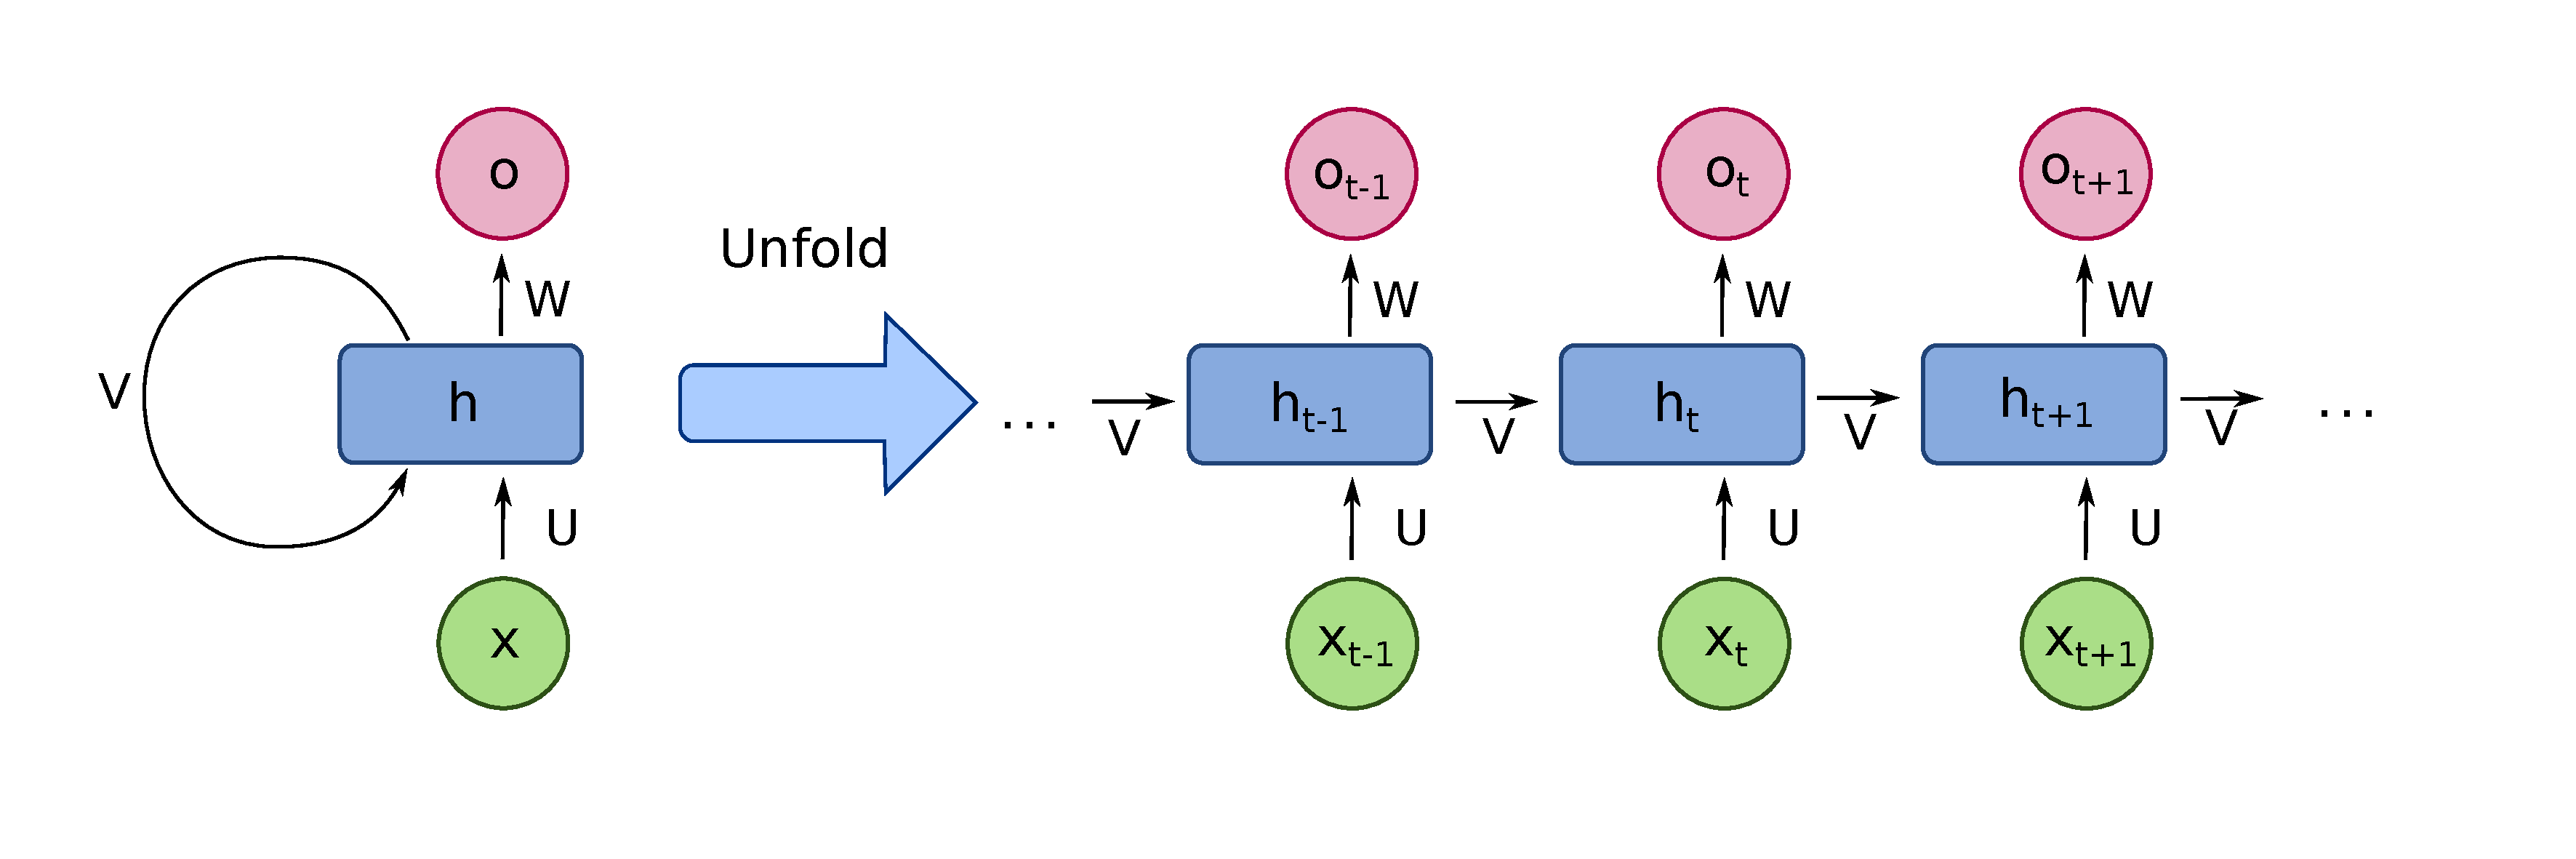
\includegraphics[width=0.95\linewidth]{images/chapter2/rnn.pdf}
	\caption{\href{https://commons.m.wikimedia.org/wiki/Artificial_neural_network} {Schemat działania rekurencyjnej sieci neuronowej z wektorem wejściowym $x$, wektorem wyjściowym $o$, wektorem stanu $h$ oraz macierzami wag $U, V, W$. Po lewej stronie przedstawiony został uprosznony model sieci, po prawej widzimy aplikację sieci dla kolejnych wektorów z sekwencji wejściowej}}
	\label{fig:rnn}
\end{figure}
\noindent Uczenie rekurencyjnej sieci neuronowej przebiega tak samo jak uczenie klasycznej sieci neuronowej, poprzez mechanizm propagacji wstecznej. Podczas uczenia sieci rekurencyjnej istnieje jednak duże ryzyko wystąpienia zjawiska zanikającego gradientu (\textit{vanishing gradient problem}) \cite{hochreiter1997long}. Problem ten może wystąpić także w klasycznych, nie rekurencyjnych sieciach neuronowych. Polega on na tym, że aktualizacje wag docierające do wcześniejszych (bliższych wejścia) warstw sieci stają się zbyt małe by znacząco zmienić jej zachowanie --- tym samym uniemożliwiając uczenie. W przypadku sieci rekurencyjnych problem jest bardziej dotkliwy, ponieważ dla przetworzenia całej sekwencji wejściowej są użyte te same wagi. Jeśli więc wagi te są mniejsze niż 1, dla wczesnych elementów sekwencji aktualizacje będą zbiegać do zera. (W przypadku wag większych niż 1, będą zbiegać do nieskończoności, co nazywane jest problemem eksplodującego gradientu). Konstrukcja LSTM opisana w następnej sekcji jest jednym ze sposobów przeciwdziałania temu zjawisku.

\subsection{Konstrukcja LSTM}

Model LSTM ma możliwość zapisania i odczytania stanu związanego z dawno przetworzonymi elementami wejściowymi. W kolejnych krokach aplikacji LSTM, oprócz dotychczasowego wyjścia przekazywany jest też wektor stanu pamięci. Po wczytaniu kolejnego elementu z sekwencji wejściowej, sieć może “zdecydować” czy odczytać informację z pamięci, czy ją nadpisać, i czy ją zresetować. Jest to zrealizowane poprzez specjalne bramki, które dla obecnego wejścia zwracają wartość 0 lub 1 (poprzez zaaplikowanie funkcji sigmoidailnej). Kolejna bramka oblicza jaką wartością nadpisać zawartość pamięci.

\subsection{Zastosowanie LSTM w przetwarzaniu języka naturalnego}

Zgodnie z jego oryginalnym przeznaczeniem, LSTM można zaaplikować do przetwarzania tekstów --- ciągów słów. Ponieważ na wejściu LSTM oczekuje sekwencji wektorów, tekst należy najpierw odpowiednio przetworzyć, na przykład za pomocą Word2Vec (Sekcja. \ref{subsec:word2vec}).

\subsection{Implementacja}

Tak jak w przypadku, wykorzystałyśmy tutaj bibliotekę \verb_keras_, poza opisanymi wcześniej funkcjami wykorzystałyśmy także dodatkową wartwę \verb_keras.layers.LSTM_. Implementuje ona rekurencyjną sieć LSTM, pozwala na zdefiniowanie wielkości wektora wyjściowego oraz prawdopodobieństwa \textit{dropoutu}.

\section{Połączenie sieci konwolucyjnej i LSTM}
\label{sec:cnn-lstm}

Częstym podejściem stosowanym w uczeniu maszynowym w celu poprawy jakości predykcji jest tzw. ensembling \cite{opitz1999popular}. Polega on na połączeniu wielu wytrenowanych modeli predykcyjnych w jeden. W publikacji \cite{minaee2019deep} autorzy opisują podejście w którym uśredniają predykcję z sieci konwolucyjnej oraz z modelu LSTM, uzyskując ostatecznie lepszy wynik na zbiorze testowym niż każdy z tych modeli z osobna.

W niniejszej pracy, podejście to zostało odtworzone za pomocą języka Python z wykorzystaniem bibliotek \verb_numpy_ oraz \verb_pandas_.

\begin{figure}[H]
	\centering
	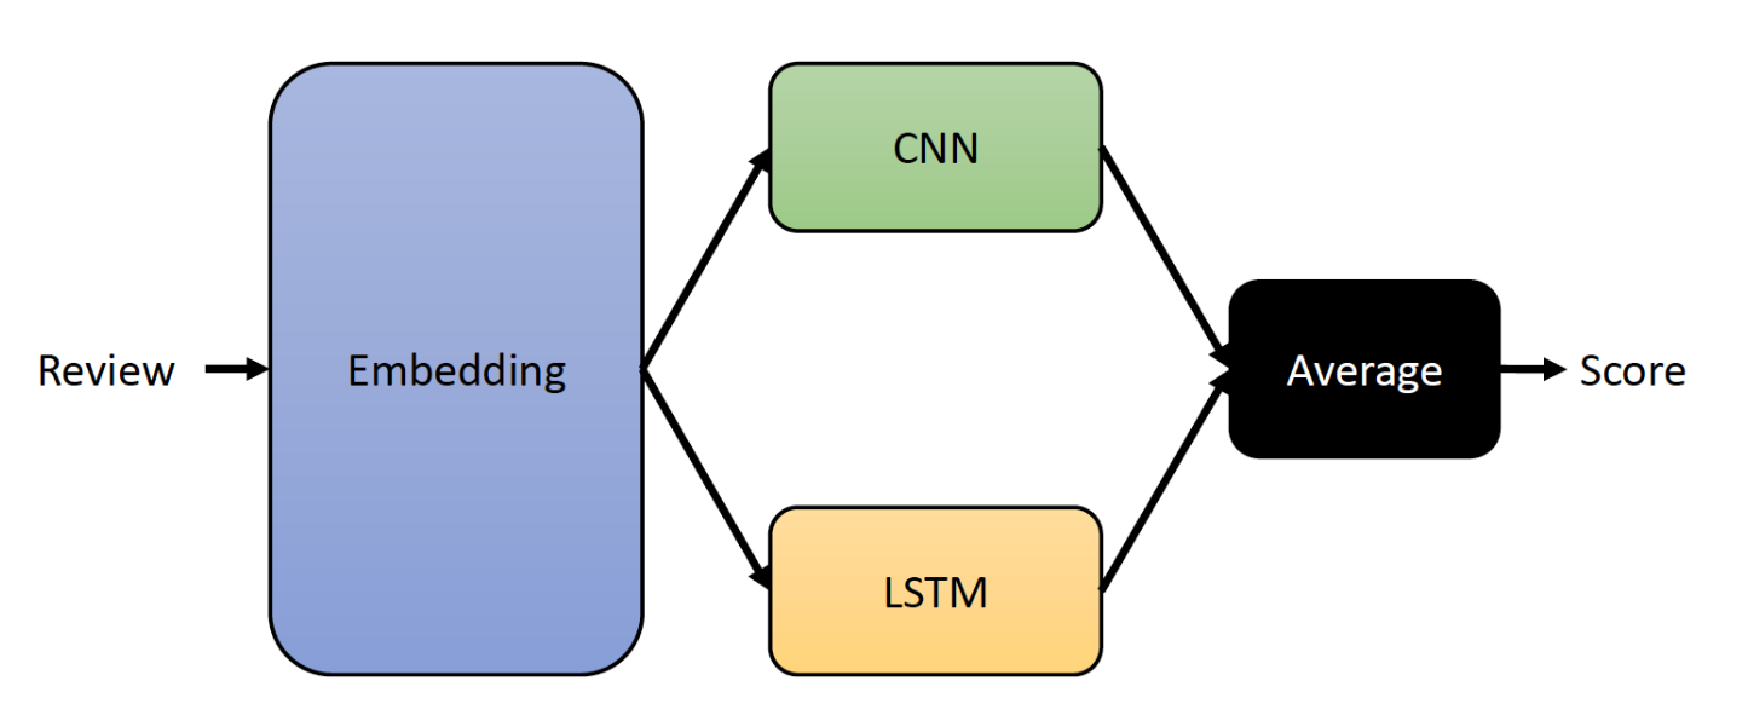
\includegraphics[width=1\linewidth]{images/chapter2/ensemble.pdf}
	\caption{Połączenie sieci konwolucyjnej i LSTM \cite{minaee2019deep}}
	\label{fig:ensemble}
\end{figure}